\chapter{Combinational Logic Building Blocks}
\addcontentsline{lobb}{chapter}{\thechapter \hspace{0.2cm} Combinational Logic Building Blocks}
\label{chapter:Combinational Building Blocks}
\graphicspath{ {./chapter04/Fig} }

In Chapter 1, Figure~\ref{fig:comboBBsys}, a digital system was defined 
as a box that transforms binary inputs to binary output.  This definition 
of a digital system was sufficient to introduce  a wide variety of 
concepts but is a handicap, now. Following is a more detailed 
definition of a digital system.
\begin{quote}  A digital system transforms the data inputs into 
data outputs.  The transformation performed by the digital system is 
specified by the control inputs.  The status outputs indicate any
exceptional events occurring during the processing of the data.
\end{quote}

Figure~\ref{fig:comboBBAsys} shows a digital system with these four types
of input and output, namely, data input, control input, data output, status output.
This classification of inputs and outputs aids in the
construction of complex digital systems using the datapath and
control methodology.

\begin{figure}[ht]
\center{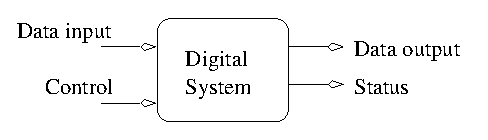
\includegraphics{Asys}}
\caption{A modified diagram of a digital system showing the classification
of the inputs and outputs.}
\label{fig:comboBBAsys}
\end{figure}

Some basic building blocks of digital systems are introduced.  
While a wide variety of blocks can be considered, those
proven to be most useful in the construction 
of digital circuits are presented.  If the right block for a particular
task does not exist, create a new block using the methods presented 
in the last chapter.  First in the examination of basic building 
blocks is a device that routes one bit of data to one of several
outputs based on an address.

\section{Decoder}

\begin{buildingblock}{Decoder}
\label{buildingblock:decoder}
\index{decoder|(}
\begin{tabular}{|l|p{3.5in}|} \hline
Nomenclature:  & N:M decoder				\\ \hline
Data Input:    & 1-bit D		\\ \hline
Data Output:   & M-bit vector $y = y_{M-1} \ldots y_1 y_0$	\\ \hline
Control:       & N-bit vector $s = s_{N-1} \ldots s_1 s_0$	\\ \hline
Status:        & none					\\ \hline
Behavior:      & $y_s = D$ all other outputs equal 0	\\ \hline
\end{tabular}
\label{page:dec}
\end{buildingblock}

To understand this definition, examine an
instance of a 3:8 decoder shown at left in Figure~\ref{fig:comboBB3:8}.
Normally, the arrows indicating the direction of the information 
flow in to and out from the decoder are not drawn.  
To understand the behavior of the decoder, its
truth table is shown to the right of Figure~\ref{fig:comboBB3:8}. 
Due to space constraints, only part of the entire truth
table is shown.

\begin{figure}[ht]
\begin{tabular}[b]{p{1.0in}p{0.5in}l}
\includegraphics[0mm,20mm][12mm,12mm]{3_8} & &
$\begin{array}{c|c|c|c||c|c|c}
s_2 & s_1 & s_0 & D & y_0 & y_1 & y_2\\ \hline
0 & 0 & 0 & 0 	& 0  &   0 &   0\\ \hline
0 & 0 & 0 & 1 	& 1  &   0 &   0\\ \hline
0 & 0 & 1 & 0 	& 0  &   0 &   0\\ \hline
0 & 0 & 1 & 1 	& 0  &   1 &   0\\ \hline
0 & 1 & 0 & 0 	& 0  &   0 &   0\\ \hline
0 & 1 & 0 & 1 	& 0  &   0 &   1\\ \hline
0 & 1 & 1 & 0 	& 0  &   0 &   0\\ \hline
0 & 1 & 1 & 1 	& 0  &   0 &   0\\ \hline
1 & 0 & 0 & 0 	& 0  &   0 &   0\\ \hline
1 & 0 & 0 & 1 	& 0  &   0 &   0\\
\end{array}$ \\
\end{tabular}
\caption{A 3:8 decoder (left) and part of its truth table (right).}
\label{fig:comboBB3:8}
\end{figure}

From the behavior listed in the description of the decoder, 
see that the $i^{th}$ output equals the data input, where
$i$ is the binary code of the select inputs.  In other
words, when $S=s_2 s_1 s_0 = 011_2 = 3_{10}$ and $D=1$,
then $y_7 y_6 y_5 y_4 y_3 y_2 y_1 y_0 = 00001000$.  If 
$S= s_2 s_1 s_0 = 011_2 = 3_{10}$ and $D=0$, then
$y_7 y_6 y_5 y_4 y_3 y_2 y_1 y_0 = 00000000$.   

The utility of this second case might be questionable because
all the outputs are the same and consequently one cannot
``see" where the output is being routed.  The resolution
to this dilemma requires considering the outputs 
through time.  A decoder is a box which sends a ``stream" of 
bits to some destination determined by the select lines.
If the destination knows that it is receiving the stream, then it
will be expecting both 1s and 0s through time.

The internal organization of a 3:8 decoder must process its four bits
of input, consisting of a 3-bit select and a 1-bit data input, and
eight bits of outputs.  In 
the previous chapter, each bit of the output could
be solved independently of the others. Hence, let's examine the $y_0$
output first.  Examination of the truth table and the behavior of
the decoder shows $y_0$ only equals 1 when
$(s_2, s_1, s_0) = (0, 0, 0)$ and $D=1$.  Borrowing the minterm
trick from page~\pageref{page:MinTrick}, $y_0=s_2's_1's_0'D$ results.
Every other output shares the characteristic that its output is
equal to 1 for a single input. Thus, each output is represented
by a minterm as shown in Figure~\ref{fig:comboBB3:8Guts}.

\begin{figure}[ht]
%% scalebox
\center{\scalebox{0.5}{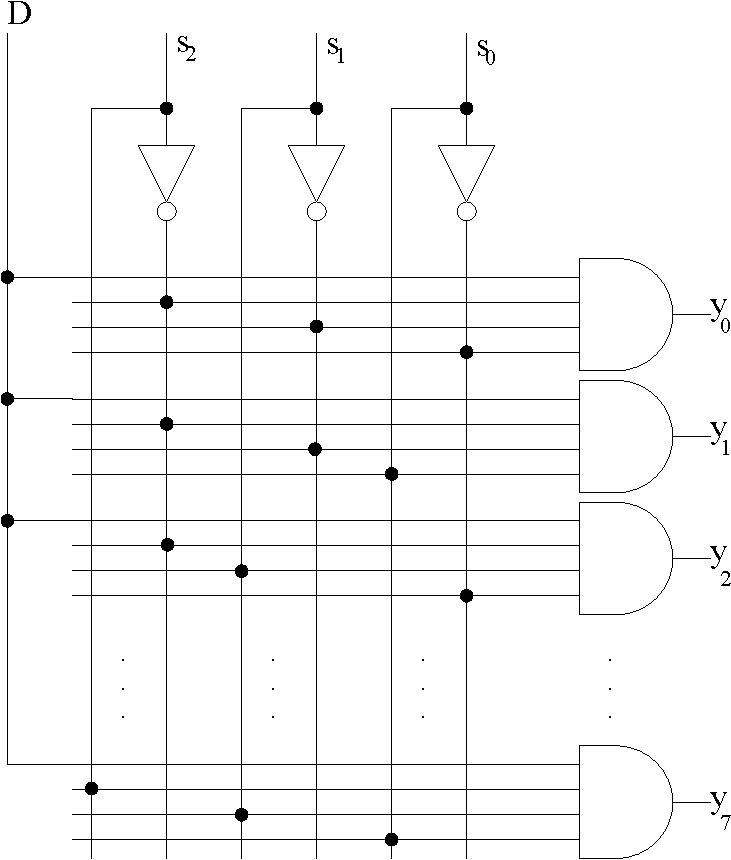
\includegraphics{3_8Guts}}}
\caption{The internal organization of a 3:8 decoder.}
\label{fig:comboBB3:8Guts}
\end{figure}

In some digital applications, the need arises to build a larger decoder
from multiple smaller decoders.  This is done by fanning-out the data input
in a tree-like structure.  The following 4:16 decoder shows how a larger decoder is
built from several smaller 2:4 decoders. 

In order to accommodate the 16 outputs, four 2:4 decoders are stacked
on top of one another as shown in Figure~\ref{fig:comboBBBigDecoder}.  These
four 2:4 decoders have a total of four bits of input.  These four bits
are sourced by the output of a single 2:4 decoder.  The
single data input of this decoder is the input of the overall 4:16
decoder.  

\begin{figure}[ht]
\center{\scalebox{0.7}{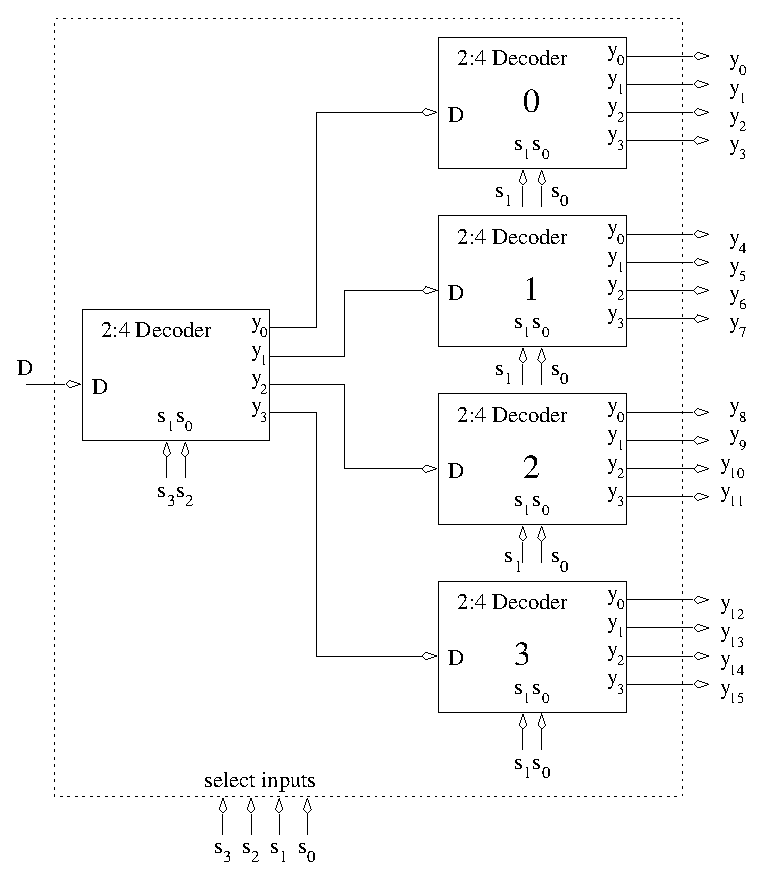
\includegraphics{BigDecoder}}}
\caption{A 4:16 decoder built from 2:4 decoders.} 
\label{fig:comboBBBigDecoder}
\end{figure}

Having organized the structure of the 2:4 decoders, all that remains 
is to route the select lines.  The outputs of the decoder labeled 
\textbf{ 3} in Figure~\ref{fig:comboBBBigDecoder} corresponds to outputs 
$y_{15} y_{14} y_{13} y_{12}$ 
of the 4:16 decoder.  Each of these outputs requires four bits of 
select with the form $s_3 s_2 s_1 s_0 = 11xx$.  Hence, $s_3 s_2 = 11$ 
must route the data input, $D$, to decoder \textbf{ 3}.  Hence, $s_3 s_2$ 
must be the select to the first level decoder in 
Figure~\ref{fig:comboBBBigDecoder}.   A similar argument for the 2:4 decoders 
labeled \textbf{ 0,1,2} reinforces the fact that $s_3 s_2$ must be the select 
to the first level decoder.  

Data routed to output $y_{12}$ has $s_3 s_2 s_1 s_0 = 1100$.  Thus, routing
at the second level of 2:4 decoders seems to be controlled by $s_1 s_0$.
Examining all the other outputs reinforces this assumption for all
the outputs.
\index{decoder|)}


\section{Multiplexer}
A multiplexer, often referred to as a mux, is data routing device 
which behaves exactly opposite of a decoder.  Its structure and
behavior is defined in the following table.

\begin{buildingblock}{Multiplexer}
\label{buildingblock:multiplexer}
\index{multiplexer|(}
\begin{tabular}{|l|p{3.5in}|} \hline
Nomenclature:  & N:1 multiplexer                        \\ \hline
Data Input:    & M-bit vector $y=y_{M-1} \ldots y_1 y_0$    \\ \hline
Data Output:   & 1-bit F          \\ \hline
Control:       & $log_2(N)$-bit vector $s = s_{log_2(N)} \ldots s_1 s_0$	\\ \hline
Status:        & none                                   \\ \hline
Behavior:      & $F = y_s$				\\ \hline
\end{tabular}
\label{page:mux}
\end{buildingblock}

To understand this definition, examine an
instance of an 8:1 mux shown on the left in Figure~\ref{fig:comboBB8:1}.
From the behavior listed in the description of the multiplexer, 
the $i^{th}$ data input is routed to the data
output where the binary code of the select inputs is $i$.
For example, if $S=s_2 s_1 s_0 = 101_2 = 5_{10}$  and 
$y_7 y_6 y_5 y_4 y_3 y_2 y_1 y_0 = 00100000$, then
$F=1$.
\\ \\
\begin{figure}[ht]
\begin{tabular}{p{1.5in}p{0.5in}l}
\includegraphics[0mm,20mm][12mm,12mm]{8_1} & &
$\begin{array}{c|c|c||c}
s_2 & s_1 & s_0 & F \\ \hline
0 & 0 & 0 & y_0 \\ \hline
0 & 0 & 1 & y_1 \\ \hline
0 & 1 & 0 & y_2 \\ \hline
0 & 1 & 1 & y_3 \\ \hline
1 & 0 & 0 & y_4 \\ \hline
1 & 0 & 1 & y_5 \\ \hline
1 & 1 & 0 & y_6 \\ \hline
1 & 1 & 1 & y_7 \\
\end{array}$
\end{tabular}
\caption{An 8:1 mux (left) and its truth table (right).}
\label{fig:comboBB8:1}
\end{figure}

The unusual form of the truth table shown in Figure~\ref{fig:comboBB8:1}
results from the fact that an 8:1 mux has a total of 11 
inputs.  There are a total of $2^{11}$ rows in this truth table
making it infeasible to list every combination of the inputs.
Consequently, in order to build an 8:1 mux, the structure of the truth table 
must be determined without
listing every combination of inputs.  Observe the $y_0$ input is routed 
to the output when 
$s_2 s_1 s_0 = 000$.  Consequently, $F=s_2' s_1' s_0' y_0$
for this input.  Each of the other outputs has a similar
minterm form.  Since only one of these ``minterms" can equal
1 for a particular select input, the minterms are ORed
together to form the output. The resulting internal 
organization of an 8:1 mux is shown in Figure~\ref{fig:comboBB8:1Guts}.

\begin{figure}[ht]
%% scalebox
\center{\scalebox{0.5}{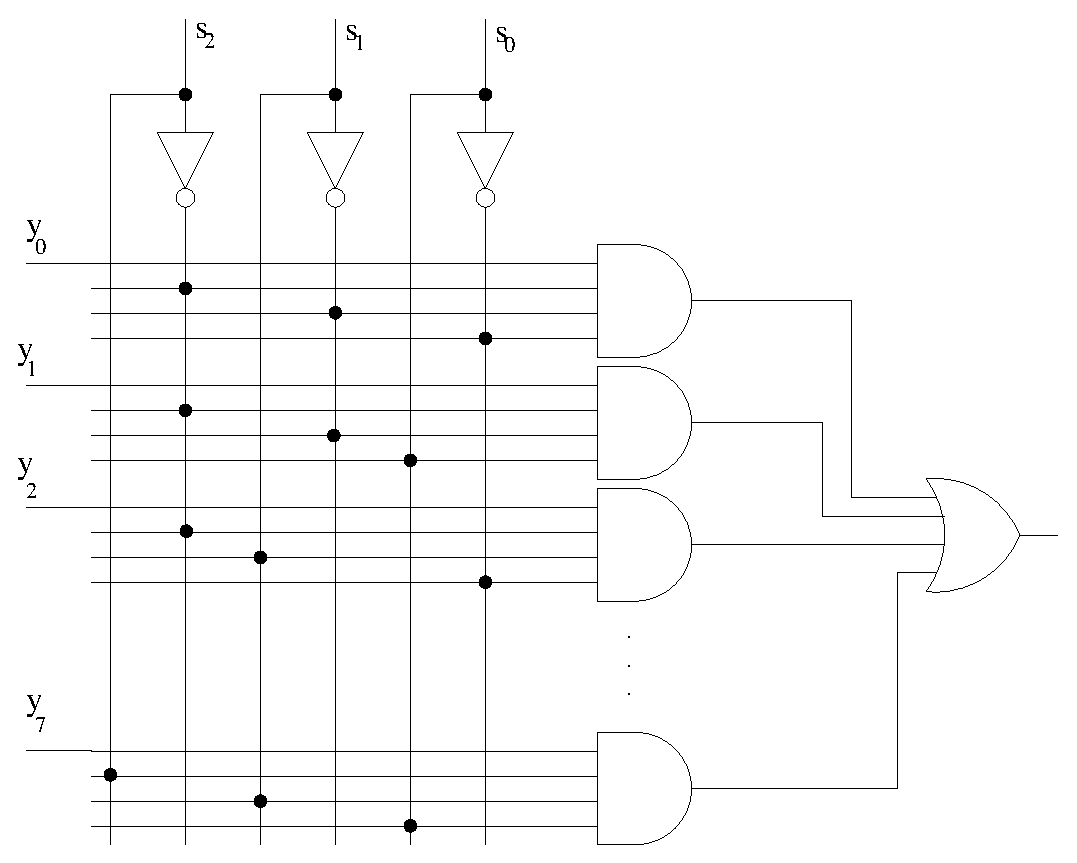
\includegraphics{8_1Guts}}}
\caption{The internal organization of an 8:1 mux.}
\label{fig:comboBB8:1Guts}
\end{figure}

As with decoders, situations arise when a larger
mux is built from smaller muxes.  The key idea is to funnel down the many data 
inputs from smaller muxes to a single output.  For example, construct 
a 16:1 mux from several 4:1 muxes.  

In order to accommodate the 16 inputs, four 4:1 muxes are stacked
on top of one another as shown in Figure~\ref{fig:comboBBBigMux}.  These
four 4:1 muxes have a total of four bits of output.  These four bits
can nicely be routed by the inputs of a single 4:1 mux.  The
single data output of this mux is the input of the overall 16:1 mux.

\begin{figure}[ht]
\center{\scalebox{0.7}{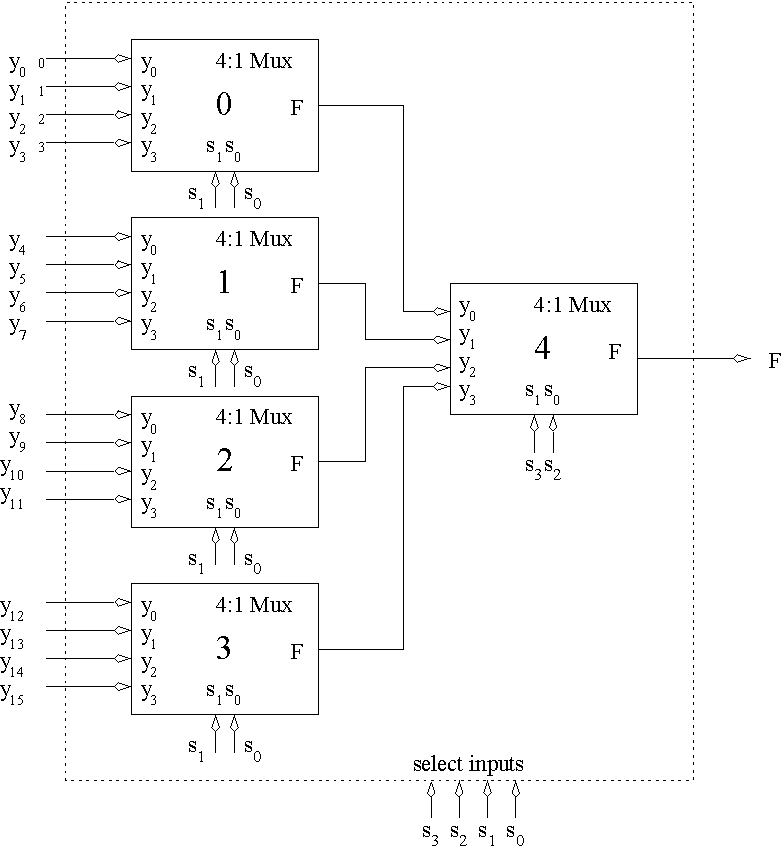
\includegraphics{BigMux}}}
\caption{The construction of a 16:1 mux from 4:1 muxes.}
\label{fig:comboBBBigMux}
\end{figure}

The select lines are assigned to the 4:1 muxes based on the following 
argument.  The inputs of the mux labeled \textbf{ 3} in
Figure~\ref{fig:comboBBBigMux} corresponds to inputs $y_{15} y_{14} y_{13} y_{12}$ 
of the 16:1 mux.  Each of these inputs requires four bits of 
select with the form $s_3 s_2 s_1 s_0 = 11xx$.  Hence, $s_3 s_2 = 11$ 
must be the select for the output mux \textbf{ 4}.  
A similar argument for the 4:1
muxes labeled \textbf{ 0,1,2} reinforces the fact that $s_3 s_2$ must be 
the select to the output mux.

In order to route $y_{12}$ to the output, the select must equal
$s_3 s_2 s_1 s_0 = 1100$.  Thus, routing at the input level of 4:1 
muxes is controlled by $s_1 s_0$.  Examining all the other 
inputs reinforces this assumption.

Occasionally the need arises to construct a mux to handle
``wide" data inputs, that is data inputs which consist of more than
a single bit.  A mux that can handle many bits is referred to 
as a \textit{ multibit mux}.  \label{multibit mux} A M-bit N:1 mux is 
defined as a N:1 mux whose data inputs and data outputs are M-bits
wide.  For example, the 4-bit 2:1 mux shown in Figure~\ref{fig:comboBB4x2x1mux} 
has two data inputs and one data output each 4-bits wide.  The internal
organization of this mux is shown on the right-hand side of 
Figure~\ref{fig:comboBB4x2x1mux}.  Four, 2:1 muxes are needed to 
accommodate all the data.  Since the data inputs are to 
be handled as a single whole, they must be routed to the
same input on each of the 2:1 muxes.
\label{page:wmu}

\begin{figure}[ht]
%% scalebox
\center{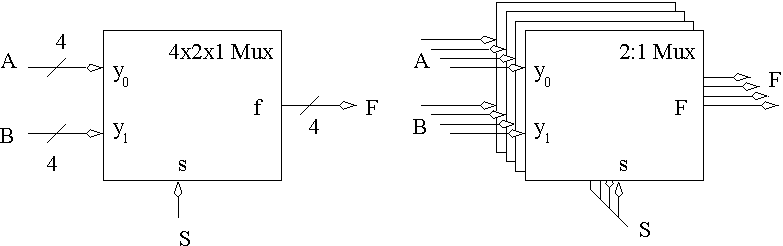
\includegraphics{4x2x1mux}}
\caption{The organization of a 4-bit 2:1 mux.  The slash labeled ``4" 
denotes the fact that these signals are 4-bits wide.}
\label{fig:comboBB4x2x1mux}
\end{figure}
\index{multiplexer|)}


\section{The Adder}
An N-bit adder is a circuit which adds two N-bit binary numbers 
$A,B$ together generating an N-bit sum $S$ and an overflow 
indication, Ovf.   

\begin{buildingblock}{Adder}
\label{buildingblock:adder}
\index{adder|(}
\begin{tabular}{|l|p{3.5in}|} \hline                    
Nomenclature:  & N-bit adder				\\ \hline
Data Input:    & two N-bit vectors $A$ and $B$		\\ \hline
Data Output:   & N-bit vector sum			\\ \hline
Control:       & none					\\ \hline
Status:        & 1-bit ovf 				\\ \hline
Behavior:      & $sum = A+B$				\\ \hline
\end{tabular}
\end{buildingblock}

The behavior of the adder is exactly as expected after reading
page~\pageref{page:addition}.  Furthermore, the overflow output is asserted 
when the adder output is greater than or equal to $2^N$.  The construction 
of an adder illustrates an approach that can be utilized for circuits 
whose function can be broken down into modular pieces. 

Approaching the design of a 4-bit adder ($N=4$) using the design 
philosophy introduced in Chapter 2, the truth table has eight bits
of inputs, 256 rows, and nine bits of outputs.  The task would be tedious,
error-prone, producing a realization with a large number of 
gates.  Instead of building the circuit as one monolithic piece, a module 
is designed that adds one set of bits together.  Four of these modules are
then connected in series to add four bits together.
For example, in Figure~\ref{fig:comboBBadd} $A=1011$ and $B=0001$ are added
together using the approach of page~\pageref{page:addition}.

\begin{figure}[ht]
\center{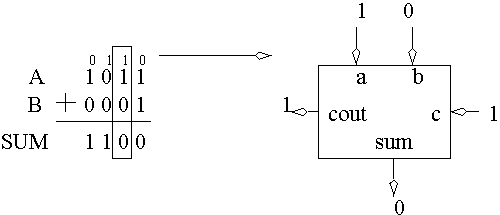
\includegraphics{add}}
\caption{An addition problem and the values of one of its
bit slices placed on a full adder.}
\label{fig:comboBBadd}
\end{figure}

This addition problem contains four \textit{ bit-slices} \index{bit-slice}.
Each bit-slice adds one bit's worth of the overall addition problem.  
The addition circuit is then constructed by stringing together four
of these bit-slice adders (called full-adders).  In the example shown
in Figure~\ref{fig:comboBBadd}, the second bit-slice of the addition problem 
is outlined.  The inputs and outputs of this bit-slice are placed on 
a full adder.  The full adder has three bits of input and two bits of output.
To build a 4-bit adder, four full adders are strung together in series
using the carry lines.  The truth table for the full adder is created 
by enumerating every combination of inputs and determining the sum and 
carry-out for each.  The carry-out and sum together are the 2-bit sum
created by adding together the three input bits.

\begin{tabular}{lp{0.5in}l}
$\begin{array}{c|c|c||c|c}
a & b & c & cout & sum \\ \hline
0 & 0 & 0 & 0 & 0 \\ \hline
0 & 0 & 1 & 0 & 1 \\ \hline
0 & 1 & 0 & 0 & 1 \\ \hline
0 & 1 & 1 & 1 & 0 \\ \hline
1 & 0 & 0 & 0 & 1 \\ \hline
1 & 0 & 1 & 1 & 0 \\ \hline
1 & 1 & 0 & 1 & 0 \\ \hline
1 & 1 & 1 & 1 & 1 \\
\end{array}$
			&
{\footnotesize
\begin{tabular}{ll}
$ \begin{array} {c||c|c|c|c}
        a \bs bc & 00 & 01 & 11 & 10 \\ \hline \hline
        0          &    &    & 1  &    \\ \hline
        1          &    & 1  & 1  & 1  \\
\end{array}$					&
$ \begin{array} {c||c|c|c|c}
        a \bs bcin & 00 & 01 & 11 & 10 \\ \hline \hline
        0          &    & 1  &    & 1  \\ \hline
        1          & 1  &    & 1  &    \\
\end{array}$ 					\\
cout = bc + a b + ac				&
sum=a b' c' + a'b'c + abc + a'bc'		\\
\end{tabular}	}
\end{tabular}


The \SOPmin expression for the outputs is arrived at by
solving Kmaps for each of the outputs.  Once, the internal
organization of a full adder is complete, four of them
are connected together as shown in Figure~\ref{fig:comboBBadder}
to build a 4-bit adder.

\begin{figure}[ht]
\center{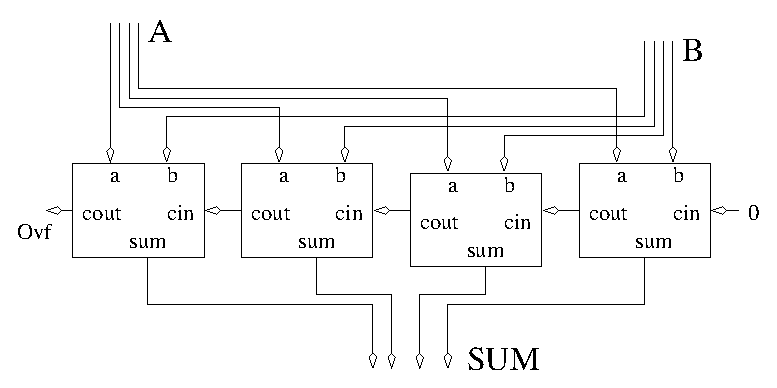
\includegraphics{adder}}
\caption{The arrangement of full adders to create a multi-bit
adder.}
\label{fig:comboBBadder}
\end{figure}
\label{page:add}

The carry-out of each bit-slice becomes the carry-in of the
next, more significant, full adder.  This sequence is necessarily
broken at the beginning and end of the chain of full 
adders.  Since there is no carry-in to the least significant
bit of an addition problem, the carry-in to the least significant
full adder is set to 0.  Since overflow occurs when the result 
of the addition process requires more bits than the word size, a 
carry-out from the most significant full adder indicates overflow.
\index{adder|)}

\section{The Adder Subtractor}

As its name implies, an adder subtractor can perform two separate
functions.  From a black-box perspective, the only difference between
this module and an adder is the presence of a control input to select
which function the adder subtractor performs.
 
\begin{buildingblock}{Adder Subtractor}
\label{buildingblock:adderSubtractor}
\index{adder subtractor|(}
\begin{tabular}{|l|p{3.5in}|} \hline
Nomenclature:  & N-bit adder subtractor                 \\ \hline
Data Input:    & two N-bit vectors $A$ and $B$           \\ \hline  
Data Output:   & N-bit vector  $s$               \\ \hline
Control:       & 1-bit $f$                     \\ \hline
Status:        & 1-bit ovf 				\\ \hline
Behavior:      & if c=0 then $s = A+B$ else $s=A-B$     \\ \hline
\end{tabular}
\end{buildingblock}

For now, assume the inputs and output of an adder subtractor are
2's-complement numbers.  Addition of 2's-complement numbers proceeds 
like the addition of regular binary numbers.  For now, 
ignore overflow conditions.  The subtraction process
for 2's-complement numbers, described on page~\pageref{page:2sub}, rewrites
the subtraction problem $A-B$ as an addition problem $A+(-B)$.  The caveat
is that $B$ must be negated.  Since both the addition and the subtraction 
problem
require an adder, all that is required is to pass either $B$ or $-B$ to the
adder depending on which operation is to be performed.  This idea is
presented in Figure~\ref{fig:comboBBAddSub}.

\begin{figure}[ht]
\center{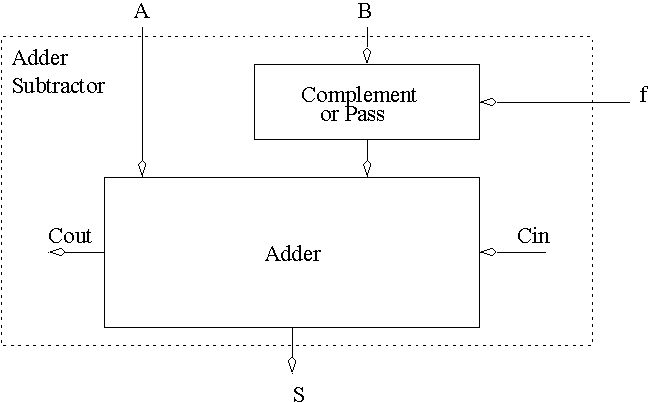
\includegraphics{AddSub}}
\caption{The idea behind the creation of an adder subtractor circuit.}
\label{fig:comboBBAddSub}
\end{figure}

The ``Complement or Pass" box in Figure~\ref{fig:comboBBAddSub} produces 
either $B$ when $f=0$ (addition) or $-B$ when $f=1$ (subtraction).
The process of complementing $B$ is to flip the bits and to add 1.
To avoid adding a second adder to perform the ``add 1" 
operation the adder shown in Figure~\ref{fig:comboBBAddSub} performs 
both $A+B$ and the ``add 1".  This little piece of magic is 
accomplished by hijacking the carry-in to the least significant 
bit of the full adder chain shown Figure~\ref{fig:comboBBadder}.  Instead
of hardwiring $cin$ shown in Figure~\ref{fig:comboBBAddSub} to 0, $cin$ is 
connected to $f$.  
When $f=1$, an extra 1 will be added to sum. The 2's-complement of
$B$ is computed in two separate steps: The ``Complement or Pass" box 
negates the bits of $B$ (when $f=1$) and the adder adds 1
(when $f=1$). Hence, the circuit performs a subtraction when $f=1$.
When $f=0$, the ``Complement or Pass" box will pass through $B$
unchanged, the adder does not add anything extra to the inputs and,
consequently, the circuit performs $A+B$.

The ``Complement or Pass" box is broken down into bit-slices, each
bit of $B$ is sent to its own slice along with the $f$ control
bit.  If $f=0$, then the slice outputs the input $B$ bit.  If $f=1$, 
then the slice outputs the complement of the $B$ bit.
The truth table is shown below.

$$\begin{array}{c|c||c}
b & f & out \\ \hline
0 & 0 & 0 \\ \hline
0 & 1 & 1 \\ \hline
1 & 0 & 1 \\ \hline
1 & 1 & 0 \\
\end{array}$$

Solving the truth table yields $out = b'f + bf' = b \oplus f$.
Each of these bit-slices is organized along with the components
in Figure~\ref{fig:comboBBAddSub} yielding the circuit diagram in
Figure~\ref{fig:comboBBTotalAddSub}.


\begin{figure}[ht]
\center{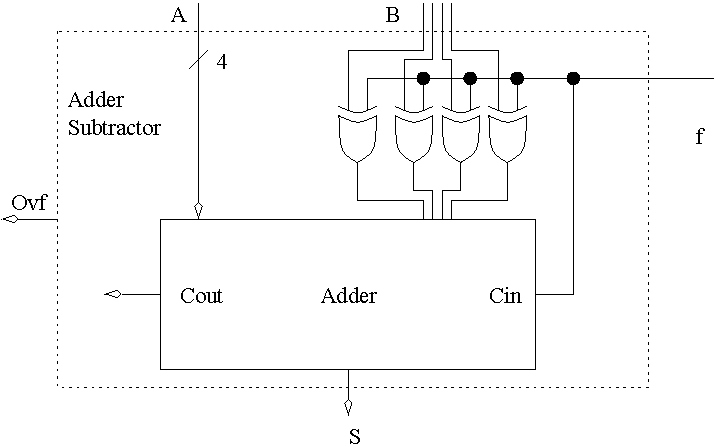
\includegraphics{TotalAddSub}}
\caption{The construction of 4-bit adder subtractor.}
\label{fig:comboBBTotalAddSub}
\end{figure}
\label{page:as}


According to page~\pageref{page:Ovf}, overflow in a 2's-complement 
operation occurs when the carry-in and carry-out to the most
significant bit-slice of the addition disagree.  In order to 
build a circuit to check this condition, the ``Adder" box shown in 
Figure~\ref{fig:comboBBTotalAddSub} must be opened revealing
the chain of full adders as shown in Figure~\ref{fig:comboBBAddSub}.
The derivation of the truth table and the circuit realization
is left as an exercise at the end of the chapter.
\index{adder subtractor|)}

\section{The Comparator}
\index{comparator|(}
A comparator is a device which determines the relative magnitude
of its two inputs.

\begin{buildingblock}{Comparator}
\label{buildingblock:comparator}

\begin{tabular}{|l|p{3.5in}|} \hline
Nomenclature:  & N-bit comparator                \\ \hline
Data Input:    & two N-bit vectors $X$ and $Y$           \\ \hline  
Data Output:   & none               \\ \hline
Control:       & none                      \\ \hline
Status:        & 1-bit $G,L,E$ \\ \hline
Behavior:      & 
		$$\begin{array}{l|l|l|l}
      			cond  & E & L & G \\ \hline
			X = Y & 1 & 0 & 0 \\ \hline
			X < Y & 0 & 1 & 0 \\ \hline
			X > Y & 0 & 0 & 1 \\
		\end{array}$$			\\ \hline
\end{tabular}
\label{page:com}
\index{comparator!truth table}
\end{buildingblock}

Comparators are rather unique because they lack data output.  That is
not to say, comparators do not have any output. Rather, their status outputs are quite
useful.  The comparator examines its two $N$-bit inputs, denoted $X$ and
$Y$, and outputs three bits describing their relative magnitudes.  
Each of these three bits, $E,L,G$, is asserted when $X$ equals $Y$, 
$X$ is less than $Y$, or $X$ is greater than $Y$, respectively.  

Much like the adder circuit the truth table method is not very 
useful for designing large comparators.  For example, a 16-bit 
comparator has two 16-bit inputs, or 32 bits of inputs, for an 
astounding $2^{32}$ rows in the truth table.  

The construction of large comparators is based on the method that 
employed to determine the relative magnitude of two numbers $X$
and $Y$, working from the most to least significant
bits.  At each step, compare a bit of $X$ and $Y$.  If the bits
are equal, then continue to the next least significant bit.  Otherwise,
either $X$ or $Y$ is larger, and the comparison is over.

Large comparators are constructed by stringing together a series
of modified 1-bit comparators as shown in Figure~\ref{fig:comboBBCompare}.  
Each bit-slice has as input a pair 
of bits from $X$ and $Y$, and $Ein$, $Gin$ and $Lin$ signals from a
more significant bit-slice.  $Ein$, $Lin$ and $Gin$ tell a bit-slice the 
status of the magnitude of $X$ and $Y$ in the bit positions to
its left.  Each bit-slice has three bits of output, $Eout$, $Lout$, and 
$Gout$, communicating the relative magnitude of the inputs so far.

\begin{figure}[ht]
\center{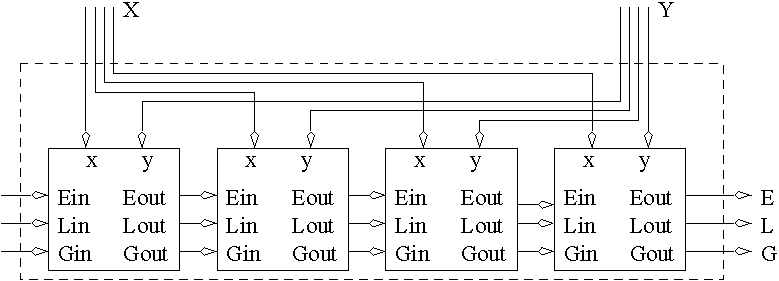
\includegraphics{Compare}}
\caption{The arrangement of the bit-slices for the comparator.}
\label{fig:comboBBCompare}
\end{figure}

The truth table for a bit-slice of the comparator has five inputs, 
$x, y, Ein, Lin$ and $Gin$.  Each bit-slice has three outputs, 
$Eout, Lout$ and $Gout$.  A portion of the truth table is shown below.

$$\begin{array}{c|c|c|c|c||c|c|c}
x & y & Ein & Lin & Gin & Eout & Lout & Gout	\\ \hline
0 & 0 & 0   & 0   & 0 	& x    & x    & x	\\ \hline
0 & 0 & 0   & 0   & 1 	& 0    & 0    & 1	\\ \hline
0 & 0 & 0   & 1   & 0 	& 0    & 1    & 0	\\ \hline
0 & 0 & 0   & 1   & 1 	& x    & x    & x	\\ \hline
0 & 0 & 1   & 0   & 0 	& 1    & 0    & 0	\\
\end{array}$$

With five bits of input, the truth table has a total of 32 rows, only
five of which are shown above.  Two rows have their outputs set to 
``don't cares" because they represent impossible situations.  The inputs
in the first row, state that the two numbers have no relative 
magnitude relative to one another.  The inputs on the fourth row 
claim that $X<Y$ and $X>Y$ simultaneously, an impossible situation.
The second row states that it has already been determined that $X>Y$,
so it does not matter what $x$ and $y$ are because their value cannot 
effect a decision that has occurred
in a more significant bit-slice.  Similarly, the third row states
that $X<Y$, so the outputs just propagate this fact, regardless 
of $x$ and $y$, because the bits of this slice are less significant
than those which decided $X<Y$.  The fifth row states that
so far $X=Y$ and since the bit-slice inputs are equal, the 
two inputs are still equal.  The remainder of the truth table will
be completed in an exercise at the end of the chapter.

The final question that must be answered is ``What should $Ein$, $Lin$,
and $Gin$, on the far left of the Figure~\ref{fig:comboBBCompare}, be assigned?"
The answer is that the $Ein, Lin,Gin$ inputs to the most significant bit-slice
should be set to 1,0,0 because $X$ and $Y$ are initially assumed to be equal.
From the preceding paragraph, observe that whenever it is determined
that $X>Y$ or $X<Y$, the comparator bit-slices will not change this 
fact.  Hence, starting the circuit off from any other initial condition
would cause an irreversible bias.  Another way to view this situation
is to realize that any binary number can be considered to have an infinite 
number of leading 0s, all of which are equal.
\index{comparator|)}



\section{Wire Logic}
\index{wire logic|(}
When  designing a digital system which contains a device
such as an adder which manipulates a pair of N-bit inputs representing
binary numbers, it is easy to forget that those N bits are really
N separate wires being grouped together.  As a
digital designer, one has access to each of these wires
and can manipulate them as necessary.  This point is important
to remember when designing with the basic building
blocks in this chapter because the number of bits representing a 
value must match the size of the device input.  For example, 
a 4-bit value cannot be run into an 8-bit-wide input and 
expected to work without some consideration of how to
handle the four, remaining bit positions.

For example, assume a 4-bit binary number 
needs to be added to an 8-bit number.  In order to 
accommodate the 8-bit number, an 8-bit
adder needs to be used.  Unfortunately, this decision creates a 
problem with the 
4-bit operand because the upper four bits of its input
are unoccupied.  The solution is to fill in the upper
four bits with 0s.  This solution is called padding with 0s 
because just like when padding is placed around an item
being shipped in a container to prevent it 
from moving around, padding a binary number with 0s 
keeps it aligned in its word-sized container. Further, the padding operation does not 
change the value of the 4-bit number.

Padding a 2's-complement number, a process called sign-extension,
is slightly more complex. Consider the problem of adding or 
subtracting a 4-bit 2's-complement number to an 8-bit 2's-complement 
number using an 8-bit adder subtractor.  The important 
point to keep in mind is that the value of the original, 4-bit, 
2's-complement must be the same as the value of the sign-extended 
8-bit 2's-complement value.  If the 4-bit value were 1111, 
representing -1 in decimal, then padding the upper four
bits with 0s would yield 00001111, which represents +15
in 8-bit 2's-complement.  This approach is not the correct way to proceed
because the original value of -1 was converted into +15 
through the sign-extension process.  Instead, the value should have been padded 
with 1s yielding 11111111, which represents -1 in an
8-bit 2's-complement number.  To show
that any negative 4-bit value padded with 1s retains its value,
show that the values of original and sign-extended 
numbers are the same when the bits are flipped and 1 is added.
Further,  any positive 4-bit value should
be padded with 0s to retain its value.  In general, the 4-bit
value needs to be padded with four copies of the most significant 
bit.

When representing a decimal value, using the base-10 numbering system, 
multiplication of a 
number by 10 can be accomplished by moving all the digits
one position to the left and inserting a 0 in the vacated
digit position.  With binary-represented values,
multiplication by 2 can be accomplished by moving all the
bits one position to the left and inserting a 0 in the 
vacated position.  This manipulation can be handled by padding the least
significant bit position with a 0.

Another useful manipulation is to combine signals together.  For 
example, consider a pair of 4-bit binary numbers
are to be added together, and their 5-bit sum is to be reported.
One alternative might be to pad each of the 4-bit inputs with a 0 and 
pass them along to a 5-bit adder.  Alternatively, 
the numbers could be used unmodified as inputs to a 4-bit adder, 
and combine the overflow output
of the 4-bit adder to the 4-bit sum output, producing a 5-bit result.
Though unconventional, this manipulation is perfectly legal and perfectly 
correct because, the overflow signal is just the 
carry-out from the most significant full adder.

\index{wire logic|)}

\section{Combinations}
The devices introduced in this section have limited utility when
used by themselves. Their real potential is realized when combined together. 
When connecting two components, the data 
outputs of one device are typically connected to the data inputs 
of other.  Likewise, the status outputs are typically connected 
to control inputs of another device.  But how are the components arranged? 
A useful starting point is to phrase the solution 
of the design problem in terms of a simple algorithm.  Algorithms 
are composed of statements. The algorithms to be constructed 
have several different types of statements.

\subsection{Arithmetic Statements}
Arithmetic statements perform the data manipulations required by
design problems.  An arithmetic statement consists of two parts,
a left-hand side (LHS) and a right-hand side (RHS), related to one
another by an equal sign.  The RHS describes the operation and its
inputs, while the LHS represents the variable denoting the output 
of the arithmetic operation.  For example, the following line of
code describes the addition of two values.

\begin{verbatim}
    x = y + 3
\end{verbatim}

The hardware realization of this line of code is an adder with \verb+y+ 
and 3 as inputs and \verb+x+ as its output.  The algorithm does not
specify the width of the \verb+x+ and \verb+y+ signals. These must
be determined from accompanying information.


\subsection{Conditional Statements}
Conditional statements arise in programming languages in the
form of \verb+if/then/else+ statements.  All conditional statements consist 
of three parts, the condition to be checked (the \verb+if+ clause), the 
statement to be evaluated when the condition is true (the \verb+then+ clause), 
and the statement to be evaluated when the condition is false (the
\verb+else+ clause).

Typically, the condition being evaluated seeks the relative
magnitude of two binary numbers.  For example, consider checking whether
 \verb+(a<4)+.  This comparison can be
realized by routing \verb+a+ and \verb+4+ into the $x$ and
$y$ inputs of a comparator and using the $L$ output.

The consequence of the condition is to cause the evaluation either of
the \verb+then+ clause or of the \verb+else+ clause.  For now, these 
clauses will 
be arithmetic statements.  In order to illustrate the hardware
realization of a conditional statement, consider the following
example.

\begin{verbatim}
    if (a<4) then x=y+3 else x=y+7
\end{verbatim}

The solution to the conditional assignment statement utilizes 
a comparator to determine the relative magnitudes of \verb+a+ 
and \verb+4+.  It is important to note in the solution shown in
Figure~\ref{fig:comboBBcond} which of the 
comparator's inputs is $x$ and $y$.  Of the three status outputs, 
the $L$ signal is used as the select on the multiplexer's inputs.  The 
other two comparator outputs should not be shown since they are
not used. 


\begin{figure}[ht]
\center{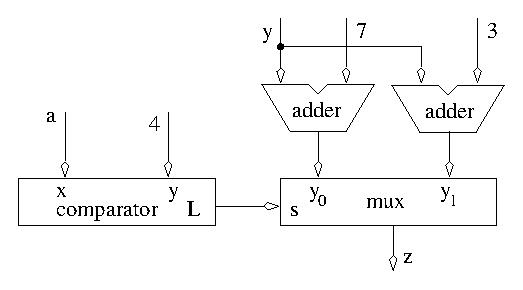
\includegraphics{cond}}
\caption{A combination of components to realize a conditional assignment
statement.}
\label{fig:comboBBcond}
\end{figure}

Each of the arithmetic operations in the algorithm is realized 
by its own adder. Notice in Figure~\ref{fig:comboBBcond} that both 
adders compute their values, and the job of the multiplexer is to 
select one of the adder outputs based on the results of the $L$ output 
from the comparator.    Since the LHS of both assignment statements
involved the same variable, the output of the mux is labeled with
$x$.  When \verb+a<4+, then 
$L=1$ and, consequently, the $y_1$ output of the mux is routed to the
output.  According to the algorithm, when \verb+a<4+, then $x=y+3$.
Consequently, $y+3$ should be routed to the $y_1$ input of the mux.
Now, only $y+7$ is left to be routed to the $y_0$ input of the mux.  It is
important to annotate the mux inputs with $y_1$ and $y_0$ in order
demonstrate that the solution works correctly.

The previous solution is more complex than it needs to be. An adder
can be removed from the circuit by noting that in the RHS of both 
assignments, the variable $y$ has either 3 or 7 added to it.  
Consequently, a mux can be used to switch through either a 3 or
7 and then to add this mux's output to $y$ as shown in 
Figure~\ref{fig:comboBBcond2}.

\begin{figure}[ht]
\center{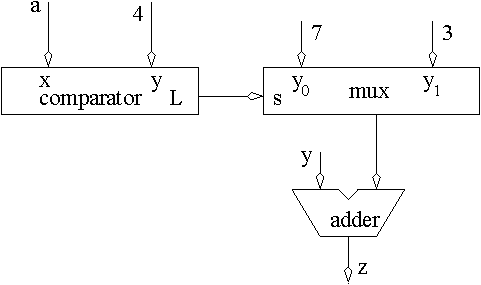
\includegraphics{cond2}}
\caption{A better realization of the conditional assignment statement.}
\label{fig:comboBBcond2}
\end{figure}

Make it a habit to identify ways to reduce the complexity
of a circuit whenever possible.  After all, one of the core
principles of engineering is always endeavor to do the most with 
the least.

